\documentclass[tikz, crop]{standalone}
\usepackage{sfmath}
\usepackage{amsmath}
\usepackage[scaled]{helvet}
\renewcommand\familydefault{\sfdefault}
\usepackage[T1]{fontenc}

\definecolor{mycolour}{RGB}{239,131,118}
\usetikzlibrary{fit,positioning,arrows.meta}

\begin{document}
\begin{tikzpicture}[
   font=\sffamily,
   arrow/.style={->,mycolour,line width=1mm},
   box/.style={mycolour,rounded corners=1mm, line width=.5mm},
   circlenode/.style={fill=mycolour, color=mycolour, line width=.75mm}
]

% Input
\node[inner sep=0pt] at (0,0) {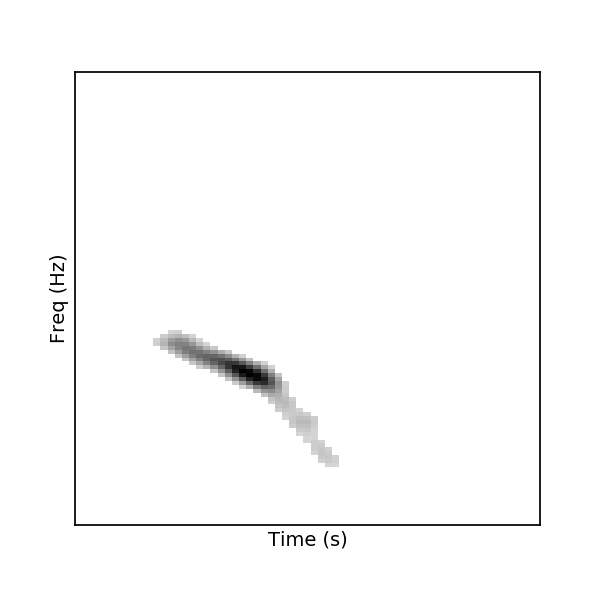
\includegraphics[width=10cm, height=10cm]{images/large_domain_spectrogram.png}};
\node[align=center, text width=4cm] at (0, 4.5) {\large Input };

% Bounding Box
\node[align=center, text width=4cm] at (-.85,0) {\small Bounding box};
\pgfmathsetmacro{\cubex}{3.25}
\pgfmathsetmacro{\cubey}{2.7}
\draw[box] (.75,-.25,0) -- ++(-\cubex,0,0) -- ++(0,-\cubey,0) -- ++(\cubex,0,0) -- cycle;
\draw[circlenode] (-2.5,-.25) circle (1mm);
\draw[circlenode] (-2.5,-2.95) circle (1mm);
\draw[circlenode] (.75,-.25) circle (1mm);
\draw[circlenode] (.75,-2.95) circle (1mm);
\draw[arrow, line width=.5mm] (.75,-1.5) -- (5.1,-1.5) node{};

% Point label and arrow
\node[align=center, text width=4cm] at (1.9,0.75)  {\large $(x_i, y_i)$};
\draw[arrow, color=black, line width=.25mm] (1.75,0.5) -- (.75,-.25) node{};

% Robot
\node[inner sep=0pt] at (6.25,-1.4) {
\includegraphics[width=2cm, height=2cm]{images/robot_emoji.png}};

% Output
\node[align=center, text width=4cm] at (9.5, 1.75) {\large Output };
\draw[arrow, line width=.5mm] (7.35,-1.5) -- (8.9,-1.5) node{};
\node[align=center, text width=4cm] at (9.5,-1) {
   \begin{equation*}
      \large
      \begin{bmatrix}
          ~?~   \\
          ~x_1~ \\
          ~x_2~ \\
          ~x_3~ \\
          ~x_4~ \\
          ~y_1~ \\
          ~y_2~ \\
          ~y_3~ \\
          ~y_4~
      \end{bmatrix}
   \end{equation*}
};

\end{tikzpicture}
\end{document}
